\documentclass[11pt]{article}

\usepackage{url}
\usepackage{hyperref}
\usepackage{graphicx}
\usepackage{verbatim}
\usepackage{color}
\setlength{\parskip}{0.5cm plus4mm minus3mm}
\usepackage{upquote}


\textwidth=6.4in
\textheight=8.5in
\hoffset=-0.7in
\voffset=-0.7in

\setlength{\parindent}{0cm} 

\newcommand{\Yfun}{Y}
%\newcommand{\TAG}{test}
\newcommand{\TAG}{\begin{color}{blue}This tutorial is currently under construction. Please check back later for more by keeping your software updated.\end{color}}

\newcommand{\HERE}{\begin{color}{blue}Currently working on this part.\end{color}}

\hyphenation{Text-Wrangler}

\title{Chapter 3: Introduction to altitude-cognizant scalar Slepian functions}
\author{The Slepian Working Group}

\usepackage{graphicx}
\graphicspath{ {./images/} }

%\userpackage{pdfpages}

\begin{document}
\maketitle

\section{Introduction}

Now that we understand the classical scalar Slepian functions, we can consider the altitude of a satellite from which the data was taken.   Atlitude-cognizant scalar Slepian functions can optimize the linear combination of spherical harmonics by either a downward continuation from the satellite radius to the planet's surface or a upward continuation from the planet's surface to the satellite radius.  The altitude-cognizant scalar Slepian functions (AC-SSF) are constructed through the maximum spherical harmonic degree L, region of concentration, planet radius, and the average satellite radius.  Since there is 'negligible' potential field in the area between the planet's surface and the satellite altitude, we optimize the potential from the planet to create a model.  The AC-SSF optimizes the linear combination of scalar spherical harmonics to incorporate the satellite altitude at which the data was taken.  Basically, we are able to take the field data collected by a satellite at some altitude and, through an optimal linear combination, we are able to plot the field on the planet's surface. 

*See Plattner and Simons 2017 for an in depth explanation.

\section{Application}

The following will include the methods for which we put Slepian functions to use.  

\subsection{Using glmalphapotup.m}
To acquire the Slepian functions, given a data set, we may use the function \verb+glmalphapotup+.  This function requires the following inputs: TH (or dom for domain), L, 

rnew -- average satellite altitude

rold -- planet radius

The outputs of this function are G, the matrix of spherical harmonic coefficients on the planet's surface, and V, the eigenvalues or the suitability factors. For all options for this function, see \verb+help glmalphapotup+.  

In our example, we will use a familiar domain, \verb+dom='africa'+ with \verb+L=10+, \verb|rnew=6371+400|, and \verb+rold=6371+.  

As mentioned in the previous chapter, we must know whether our spherical harmonic coefficients are in ADDMOUT or ADDMON ordering.  By using the \verb+help+ function, it is clear that the output is in ADDMOUT ordering; this will be useful information in a moment.  So, we can run:

\verb+[G,V] = glmalphapotup(dom,L,rnew,rold);+

\subsection{Plotting}
However, to plot the Slepian function at satellite altitude, we must upward continue the functions by using the function \verb+potup+.  This requires the inputs: G, radius to the satellite, planet radius, and L.  

\subsubsection{Example One:}
For this example, we will use the spherical harmonic coefficient for the optimal Slepian function, which would be the first column of G.  We can now run:

\verb+coef = potup(G(:,1),rnew,rold,L,1);+

providing the output of the spherical harmonic coefficient vector for radial field at the new altitude.

To plot the Slepian functions on the surface of the planet, we may use the same functions as in the previous chapter, for the classical scalar Slepian functions: \verb+plm2xyz+ and \verb+plotplm+.  Before this, however, we will need to convert our G into lmcosi, since G is in ADDMOUT, so run:

\verb+lmcosi = coef2lmcosi(coef,1);+

Now set the resolution to \verb+res=1+ and convert the coefficients to xyz coordinates by running:

\verb+data = plm2xyz(lmcosi,res);+

Finally, to plot the figure on a flat surface, run:

\verb+plotplm(data,[],[],4,res)+

Let's add a color bar and make the color scale nicer by running:

\verb+colorbar+\\
\verb+caxis([-1,1]*max(abs(caxis)))+\\
\verb+kelicolor(1)+

To plot the figure on a 3-D sphere, run:

\verb+plotplm(lmcosi,[],[],2,res)+

For the results, see Figure 1.
\begin{figure}
  \centering
  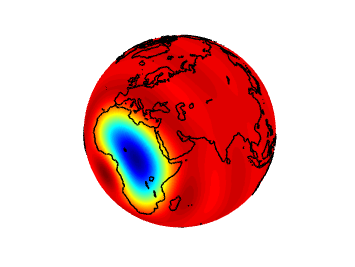
\includegraphics[width=0.5\textwidth]{ch3plot.png}
  \caption{Result of plotplm with G(:,1).}
\label{plotplm}
\end{figure}

\textbf{Exercise:} Let's try another region, say a spherical cap:

\verb+dom = [16]+

Run every step above again.  What is the result?  Compare to figure....

\textbf{Exercise:} We can try another region, say a spherical ring:

\verb+dom = [100,25]+

What is the result? Compare to figure......

See the \verb+help+ function to see what other regions we can choose for \verb+glmalphapotup+.

\subsection{Linear combinations of Slepian functions}

Now that we know how to create and plot the Slepain functions at satellite altitude with different regions, we can create a linear combination of the altitude-cognizant Slepian functions.  What does the linear combination \verb|g{1}=G(:,1)+3G(:,2)| look like?  You will need to input this linear combination into your command line and run the same process, with \verb+g{1}+ instead of \verb+G(:,1)+ in the functions:

\verb+coef = potup(g{1},rnew,rold,L,1);+\\
\verb+lmcosi = coef2lmcosi(coef,1);+\\
\verb+plot(lmcosi,[],[],2,res)+

This should result in figure 2.

\textbf{Exercise:} Try some of your own linear combinations.

\subsubsection{Example Two:}
Now, let's try a set of linear combinations including all of the spherical harmonic coefficients in our case.  The length of our matrix, G, is $(L+1)^2$.  Let:

\verb|K = length(G)|

We need to determine a proper value for \verb+J+ to plot the optimal linear combination of Slepian functions.  We will first need to plot our index \verb+j+ versus \verb+V+:

\verb|plot(1:K,V)|

Now we can analyze the plot to determine which value of J such that most of the eigenvalues are concentrated within our region.  Our plot will look like figure.... , as an exponential decay curve.  By analyzing the graph, it looks like the eigenvalues near zero at about $J=50$.  You will have to manually choose your J value, so run:

\verb+J = 50+

We will need to use a \verb+for+ loop to run through all the spherical harmonic coefficients contained in the matrix \verb+G+, with \verb+J+ columns.  Combining our knowledge from above, run:

\verb+for j=1:J+\\
\verb+    g{j} = plm2xyz(coef2lmcosi(potup(G(:,j),rnew,rold,L,1),1),res);+\\
\verb+end+

This gathers all of the coefficients into a cell array, \verb+g{j}+, while sorting them into the appropriate format.  Now we can choose some random values:

\verb+u = rand(J,1);+

Now, we need to create a matrix, \verb+f+, which is the same size as our coefficients. Run:

\verb+f = zeros(size(g{1}));+

Finally, we can build our linear combination of spherical harmonics, which describe the Slepian functions:

\verb+for j=1:J+\\
\verb|    f = f+u(j)*g{j};|\\   
\verb+end+

Again, use \verb+plotplm+ to plot and adjust the color:

\verb+plotplm(f,[],[],4,res)+\\
\verb+kelicol(1)+\\
\verb+caxis([-1,1]*max(abs(caxis)))+

Compare your plot to figure 3.  As  you can see, the Slepian functions are describing the region chosen, \verb|'africa'|.  

\textbf{Question:} Choose a lower J value and compare the plots.  What do you notice?



\textit{**This chapter is currently under construction.**}

\end{document}